\section{Introduction}


%%%%%%%%%%%%%%%%%%%%%%%%%%%%%%%%%%%%%%%%%%%%%%%%%%%%%%%%%%%%%%%%%%%%%%%%%%%%%%%
\section{Methodology}

Starting with \citet{Thompson1982} and \citet{Reid1990}, Euler's equation has
been used to estimate the source positions of gravity and magnetic data.
In this section, we will review the solution of Euler's equation for
$(x_o, y_o, z_o)$ by Euler deconvolution \citep{Reid1990} and then present a
new method, called \textit{Euler inversion}, for solving Euler's equation using
total least-squares.

We start with Euler's homogeneity equation

\begin{equation}
  (x - x_o)\partial_x f + (y - y_o)\partial_y f + (z - z_o)\partial_z f
  + \eta(f - b) = 0
  \ ,
  \label{eq:euler}
\end{equation}

\noindent
in which $f$ is a homogeneous function (in this case, a potential-field),
$\partial_\alpha$ is the derivative operator in the $\alpha$ dimension,
$(x, y, z)$ are the coordinates of the observation point,
$(x_o, y_o, z_o)$ are the coordinates of the field source,
$b$ is the base level representing a constant shift in the field,
and $\eta$ is the structural index, which is related to the nature of the
source and how its potential-field values decay with distance
\citep{Ruddock1966,Reid2014}.
Equation~\ref{eq:euler} relates the coordinates of the source with the
potential field and its gradient observed at the point $(x, y, z)$.

Given $N$ observations points in which we have measured $f$ and its gradient
(for a total $4N$ data), we can define the system of $N$ equations and $4$
unknowns

\begin{equation}
  \begin{aligned}
    (x_1-x_o)\partial_x f_1 + (y_1-y_o)\partial_y f_1 + (z_1-z_o)\partial_z f_1 + \eta(f_1-b) &= 0
    \\
    (x_2-x_o)\partial_x f_2 + (y_2-y_o)\partial_y f_2 + (z_2-z_o)\partial_z f_2 + \eta(f_2-b) &= 0
    \\
    \vdots
    \\
    (x_N-x_o)\partial_x f_N + (y_N-y_o)\partial_y f_N + (z_N-z_o)\partial_z f_N + \eta(f_N-b) &= 0
  \end{aligned}
  \ .
  \label{eq:euler-system}
\end{equation}

\noindent
Both Euler deconvolution and Euler inversion aim to solve the equation system
above to estimate the parameter vector

\begin{equation}
  \mathbf{p} = \begin{bmatrix}x_o & y_o & z_o & b \end{bmatrix}^T.
  \label{eq:p}
\end{equation}


\subsection{Euler deconvolution}

Euler deconvolution starts by rearranging Equation~\ref{eq:euler-system} to
place the parameters on the left-hand side and all other terms on the
right-hand side. This is an attempt to form a \textit{parametric model} which
results in the equation system

\begin{equation}
  \begin{aligned}
  -x_o\partial_x f_1 - y_o\partial_y f_1 - z_o\partial_z f_1 - \eta b &= -x_1\partial_x f_1 - y_1\partial_y f_1 - z_1\partial_z f_1 - \eta f_1
  \\
  -x_o\partial_x f_2 - y_o\partial_y f_2 - z_o\partial_z f_2 - \eta b &= -x_2\partial_x f_2 - y_2\partial_y f_2 - z_2\partial_z f_2 - \eta f_2
  \\
  \vdots
  \\
  -x_o\partial_x f_N - y_o\partial_y f_N - z_o\partial_z f_N - \eta b &= -x_N\partial_x f_N - y_N\partial_y f_N - z_N\partial_z f_N - \eta f_N
  \end{aligned}
  \ ,
\end{equation}

\noindent
which can be written in matrix form as

\begin{equation}
  \underbrace{
    \begin{bmatrix}
      -\partial_x f_1 & -\partial_y f_1 & -\partial_z f_1 & -\eta \\
      -\partial_x f_2 & -\partial_y f_2 & -\partial_z f_2 & -\eta \\
      \vdots & \vdots & \vdots & \vdots \\
      -\partial_x f_N & -\partial_y f_N & -\partial_z f_N & -\eta
    \end{bmatrix}
  }_{\mathbf{A}}
  \underbrace{
    \begin{bmatrix}
      x_o \\ y_o \\ z_o \\ b
    \end{bmatrix}
  }_{\mathbf{p}}
  =
  \underbrace{
    \begin{bmatrix}
      -x_1\partial_x f_1 - y_1\partial_y f_1 - z_1\partial_z f_1 - \eta f_1 \\
      -x_2\partial_x f_2 - y_2\partial_y f_2 - z_2\partial_z f_2 - \eta f_2 \\
      \vdots \\
      -x_N\partial_x f_N - y_N\partial_y f_N - z_N\partial_z f_N - \eta f_N \\
    \end{bmatrix}
  }_{\mathbf{c}}
  \ ,
  \label{eq:deconv-system}
\end{equation}

\noindent
in which $\mathbf{A}$ is the Jacobian matrix of Euler's equation
(Equation~\ref{eq:euler}) with respect to the parameters
(Equations~\ref{eq:p})
and $\mathbf{c}$ is a \textit{pseudo-data vector}.

The solution proposed by \citet{Thompson1982} and \citet{Reid1990} is a
least-squares estimate of $\mathbf{p}$

\begin{equation}
  \hat{\mathbf{p}} = \left(\mathbf{A}^T\mathbf{A}\right)^{-1}
  \mathbf{A}^T\mathbf{c}
  \ .
  \label{eq:deconv-p}
\end{equation}

\noindent
The covariance matrix of the solution $\mathbf{C}_p$ is obtained through
standard error propagation assuming that the only variable with uncertainty
is the pseudo-data vector $\mathbf{c}$

\begin{equation}
  \mathbf{C}_p = \hat{\sigma}_0^2 \left(\mathbf{A}^T\mathbf{A}\right)^{-1}
  \ ,
  \label{eq:deconv-cov}
\end{equation}

\noindent
in which
${\hat{\sigma}_0^2} = \|\mathbf{c} - \mathbf{A}\mathbf{p}\|^2 / (N - 4)$
is the reduced chi-squared statistic and an estimate of the variance factor of
$\mathbf{c}$.

The solution in Equation~\ref{eq:deconv-p} above is valid only if the
contents of the Jacobian matrix $\mathbf{A}$ are assumed to be error-free.
As can be seen from Equation~\ref{eq:deconv-system}, the Jacobian contains the
derivatives of $f$, which are often computed numerically by finite-differences
or Fourier transforms and are known to amplify the high-frequency random noise
in the data.
This presents a problem, particularly for the estimation of $z_o$, which has
been widely explored in the literature
\citep{Silva2001,Melo2020,Pasteka2009,Florio2014}.


\subsection{Euler inversion: Formulation}

Euler inversion starts by assigning the potential-field $f$ to a $N \times 1$
vector

\begin{equation}
  \mathbf{f} =
  \begin{bmatrix}
    f_1 & f_2 & \cdots & f_N
  \end{bmatrix}^T.
\end{equation}

\noindent
We can then define a $4N \times 1$ \textit{data vector} which contains all of
the values of $f$ and its gradient

\begin{equation}
  \mathbf{d} =
  \begin{bmatrix}
    \mathbf{f}^T
    & \mathbf{\nabla}_x\mathbf{f}^T
    & \mathbf{\nabla}_y\mathbf{f}^T
    & \mathbf{\nabla}_z\mathbf{f}^T
  \end{bmatrix}^T.
  \label{eq:d}
\end{equation}

\noindent
in which $\mathbf{\nabla}_\alpha$ is the gradient operator in the $\alpha$
dimension.

Next, we formulate the $N \times 4$ equation system from Euler's equation as a
non-linear function of parameters and data

\begin{equation}
  \mathbf{e}(\mathbf{p}, \mathbf{d}) = \mathbf{0}
  \ ,
  \label{eq:e}
\end{equation}

\noindent
which is known in geodesy as an \textit{implicit model} \citep{Vanicek1986}.

We then wish to solve the following constrained optimization problem with
non-linear equality constraints to estimate both the parameters and the
predicted data simultaneously

\begin{equation}
  \begin{aligned}
    \min_{\mathbf{p}, \mathbf{d}} \quad &
      \phi(\mathbf{d}) =
      \left[\mathbf{d}^o - \mathbf{d}\right]^T \mathbf{W}
      \left[\mathbf{d}^o - \mathbf{d}\right]
    \\
    \textrm{subject to} \quad &
      \mathbf{e}(\mathbf{p}, \mathbf{d}) = \mathbf{0}
    \ ,
  \end{aligned}
  \label{eq:constrained}
\end{equation}

\noindent
in which $\mathbf{d}^o$ is the \textit{observed data vector} which contains all
of the $4N$ observations of $f$ and its gradient,
$\mathbf{d}$ is the \textit{predicted data vector} from Equation~\ref{eq:d},
and $\mathbf{W}$ is a $4N \times 4N$ diagonal weight matrix.
The first $N$ terms of the diagonal of $\mathbf{W}$ are the weights for the
potential field observations and the following $3N$ terms are the weights of
x-, y-, and z-derivatives of the potential field, in order.

The constrained problem in Equation~\ref{eq:constrained} can be transformed
into an unconstrained problem by using the Lagrangian

\begin{equation}
  \Lagr(\mathbf{p}, \mathbf{d}, \boldsymbol{\lambda}) =
    \left[\mathbf{d}^o - \mathbf{d}\right]^T \mathbf{W}
    \left[\mathbf{d}^o - \mathbf{d}\right]
    +
    2 \boldsymbol{\lambda}^T \mathbf{e}
  \ ,
  \label{eq:lagrangian}
\end{equation}

\noindent
in which $\boldsymbol{\lambda}$ is an $N \times 1$ vector of Lagrange
multipliers.
The non-linear Lagrangian is minimized through Newton's method
\citep{Aster2018}.
We start with initial estimates $\mathbf{p}_0$ and $\mathbf{d}_0$ and then
iteratively apply corrections $\mathbf{\Delta p}_k$ and $\mathbf{\Delta d}_k$
until convergence is achieved.
To calculate the corrections, we introduce a new variable $\mathbf{u} =
[\mathbf{d}^T\  \boldsymbol{\lambda}^T \ \mathbf{p}^T]^T$, expand the
Lagrangian $\Lagr(\mathbf{u})$ (Equation~\ref{eq:lagrangian}) in a Taylor
series around point $\mathbf{u}_k$, and disregard terms of order higher than
two

\begin{equation}
  \Lagr(\mathbf{u}) \approx
  \Gamma(\mathbf{u}) =
  \Lagr(\mathbf{u}_k)
    + \mathbf{\Delta u}_k^T \mathbf{\nabla}\Lagr(\mathbf{u}_k)
    + \dfrac{1}{2}\mathbf{\Delta u}_k^T\mathbf{H}_k\mathbf{\Delta u}_k
  \ ,
  \label{eq:taylor}
\end{equation}

\noindent
in which $\mathbf{\nabla}$ is the gradient operator and $\mathbf{H}_k$ is the
Hessian matrix of $\Lagr$ evaluated at $\mathbf{u}_k$.
Equation~\ref{eq:taylor} is a quadratic function of $\mathbf{\Delta u}_k$ and
we can obtain its minimum by taking its gradient and equating it to the null
vector

\begin{equation}
  \begin{gathered}
    \mathbf{\nabla}\Gamma(\mathbf{\Delta u}_k) =
      \mathbf{\nabla}\Lagr(\mathbf{u_k})
      + \mathbf{H}_k\mathbf{\Delta u}_k
      = \mathbf{0}
    \ ,
    \\
    \mathbf{H}_k\mathbf{\Delta u}_k = -\mathbf{\nabla}\Lagr(\mathbf{u_k})
    \ .
  \end{gathered}
\end{equation}

\noindent
The equation above is the \textit{system of normal equations}, which can also
be written in terms of $\mathbf{p}$, $\boldsymbol{\lambda}$, and $\mathbf{d}$

\begin{equation}
  \underbrace{
    \begin{bmatrix}
      \mathbf{H}^{dd}_k & \mathbf{H}^{d\lambda}_k & \mathbf{H}^{dp}_k \\
      \mathbf{H}^{\lambda d}_k & \mathbf{H}^{\lambda\lambda}_k & \mathbf{H}^{\lambda p}_k \\
      \mathbf{H}^{pd}_k & \mathbf{H}^{p\lambda}_k & \mathbf{H}^{pp}_k
    \end{bmatrix}
  }_{\text{Hessian of }\Lagr}
  \underbrace{
    \begin{bmatrix}
      \mathbf{\Delta d}_k \\
      \boldsymbol{\Delta\lambda}_k \\
      \mathbf{\Delta p}_k
    \end{bmatrix}
  }_{\mathbf{\Delta u}_k}
  = -
  \underbrace{
    \begin{bmatrix}
      \mathbf{\nabla}_d\Lagr(\mathbf{p}_k,\mathbf{d}_k,\boldsymbol{\lambda}_k) \\
      \mathbf{\nabla}_\lambda\Lagr(\mathbf{p}_k,\mathbf{d}_k,\boldsymbol{\lambda}_k) \\
      \mathbf{\nabla}_p\Lagr(\mathbf{p}_k,\mathbf{d}_k,\boldsymbol{\lambda}_k)
    \end{bmatrix}
  }_{\text{gradient of }\Lagr}
  \ ,
\end{equation}

\noindent
in which $\mathbf{\nabla}_\alpha$ is the gradient operator with respect to
variable $\alpha$ and
$\mathbf{H}_k^{\alpha\beta}$ is the Hessian matrix of $\Lagr$ with respect to
variables $\alpha$ and $\beta$, evaluated at $\mathbf{u}_k$.
Since the order of derivation can be swapped in the Hessian matrices and the
Hessian of $\Lagr$ is symmetric, the above equation can be simplified to

\begin{equation}
    \begin{bmatrix}
      \mathbf{H}^{dd}_k & \mathbf{H}^{d\lambda}_k & \mathbf{H}^{dp}_k \\
      {\mathbf{H}^{d\lambda}_k}^T & \mathbf{H}^{\lambda\lambda}_k & \mathbf{H}^{\lambda p}_k \\
      {\mathbf{H}^{dp}_k}^T & {\mathbf{H}^{\lambda p}_k}^T & \mathbf{H}^{pp}_k
    \end{bmatrix}
  \begin{bmatrix}
    \mathbf{\Delta d}_k \\
    \boldsymbol{\Delta\lambda}_k \\
    \mathbf{\Delta p}_k
  \end{bmatrix}
  = -
    \begin{bmatrix}
      \mathbf{\nabla}_d\Lagr(\mathbf{p}_k,\mathbf{d}_k,\boldsymbol{\lambda}_k) \\
      \mathbf{\nabla}_\lambda\Lagr(\mathbf{p}_k,\mathbf{d}_k,\boldsymbol{\lambda}_k) \\
      \mathbf{\nabla}_p\Lagr(\mathbf{p}_k,\mathbf{d}_k,\boldsymbol{\lambda}_k)
    \end{bmatrix}
  \ .
  \label{eq:newton}
\end{equation}

Now, we must derive the three gradient vectors and six Hessian matrices in
Equation~\ref{eq:newton}.
We will start with the gradient vectors.

\begin{equation}
  \begin{aligned}
    \mathbf{\nabla}_d\Lagr(\mathbf{p}_k,\mathbf{d}_k,\boldsymbol{\lambda}_k) &=
      2\left(-\mathbf{W}\left[\mathbf{d}^o - \mathbf{d}_k\right]
      + \mathbf{B}_k^T\boldsymbol{\lambda}_k\right)
    \ ,
    \\
    \mathbf{\nabla}_\lambda\Lagr(\mathbf{p}_k,\mathbf{d}_k,\boldsymbol{\lambda}_k) &=
      2\mathbf{e}_k
    \ ,
    \\
    \mathbf{\nabla}_p\Lagr(\mathbf{p}_k,\mathbf{d}_k,\boldsymbol{\lambda}_k) &=
      2\mathbf{A}_k^T\boldsymbol{\lambda}_k
    \ ,
  \end{aligned}
  \label{eq:grad}
\end{equation}

\noindent
in which $\mathbf{e}_k = \mathbf{e}(\mathbf{p}_k,\mathbf{d}_k)$
(Equation~\ref{eq:e}), $\mathbf{A}_k$ is the $N \times 4$ \textit{parameter
Jacobian} matrix of Euler's equation (Equation~\ref{eq:deconv-system})
evaluated on $(\mathbf{p}_k,\mathbf{d}_k)$, and $\mathbf{B}_k$ is the $N \times
4N$ \textit{data Jacobian} of Euler's equation, also evaluated on
$(\mathbf{p}_k,\mathbf{d}_k)$, which is composed of four diagonal matrices

\begin{equation}
  \mathbf{B}_k =
  \begin{bmatrix}
    \mathbf{B}^f_k &
    \mathbf{B}^x_k &
    \mathbf{B}^y_k &
    \mathbf{B}^z_k
  \end{bmatrix}
  \ .
  \label{eq:B}
\end{equation}

\noindent
The diagonal elements of each of the four matrices are

\begin{equation}
  \begin{aligned}
    {B^f_k}_{ii} &= \eta \ , &
    {B^x_k}_{ii} &= x_i - {x_o}_k \ , &
    {B^y_k}_{ii} &= y_i - {y_o}_k \ , &
    {B^z_k}_{ii} &= z_i - {z_o}_k \ .
  \end{aligned}
\end{equation}

The Hessian matrices are calculated using a Gauss-Newton approximation
disregarding second-order derivatives. The six independent Hessians are given
by

\begin{equation}
  \begin{aligned}
    \mathbf{H}^{dd}_k &\approx 2\mathbf{W} \ , &
    \mathbf{H}^{\lambda\lambda}_k &= \mathbf{0} \ , &
    \mathbf{H}^{pp}_k &\approx \mathbf{0} \ ,
    \\
    \mathbf{H}^{d\lambda}_k &= 2\mathbf{B}^T \ , &
    \mathbf{H}^{\lambda p}_k &= 2\mathbf{A} \ , &
    \mathbf{H}^{dp}_k &\approx \mathbf{0} \ .
  \end{aligned}
  \label{eq:hess}
\end{equation}

\noindent
Substituting the gradients (Equation~\ref{eq:grad}) and Hessians
(Equation~\ref{eq:hess}) into the system of normal equations of Newton's method
(Equation~\ref{eq:newton}) we arrive at

\begin{equation}
    \begin{bmatrix}
      \mathbf{W} & \mathbf{B}_k^T & \mathbf{0} \\
      \mathbf{B}_k & \mathbf{0} & \mathbf{A}_k \\
      \mathbf{0} & \mathbf{A}_k^T & \mathbf{0}
    \end{bmatrix}
  \begin{bmatrix}
    \mathbf{\Delta d}_k \\
    \boldsymbol{\Delta\lambda}_k \\
    \mathbf{\Delta p}_k
  \end{bmatrix}
  = -
    \begin{bmatrix}
      -\mathbf{W}\left[\mathbf{d}^o - \mathbf{d}_k\right] + \mathbf{B}_k^T\boldsymbol{\lambda}_k
      \\
      \mathbf{e}_k
      \\
      \mathbf{A}_k^T\boldsymbol{\lambda}_k
    \end{bmatrix}
  \ .
  \label{eq:normal}
\end{equation}

Since the data weight matrix $\mathbf{W}$ is diagonal and invertible, we can
use the following identity to eliminate one equation from the equation system
above \citep{WellsKrakiwsky1971}

\begin{equation}
    \begin{bmatrix}
      \mathbf{C} & \mathbf{D} \\
      \mathbf{E} & \mathbf{F}
    \end{bmatrix}
    \begin{bmatrix}
      \mathbf{g} \\
      \mathbf{h}
    \end{bmatrix}
    +
    \begin{bmatrix}
      \mathbf{t}
      \\
      \mathbf{v}
    \end{bmatrix}
    =
    \begin{bmatrix}
      \mathbf{0}
      \\
      \mathbf{0}
    \end{bmatrix}
    \ \Rightarrow \
    \left[\mathbf{F} - \mathbf{E}\mathbf{C}^{-1}\mathbf{D}\right]\mathbf{h}
    + \mathbf{v} - \mathbf{E}\mathbf{C}^{-1}\mathbf{t} = \mathbf{0}
  \ .
  \label{eq:identity}
\end{equation}

Applying the identity to Equation~\ref{eq:normal} with
$\mathbf{g} = \mathbf{\Delta d}_k$ and
$\mathbf{h} = \left[\boldsymbol{\Delta\lambda}_k \quad \mathbf{\Delta p}_k\right]^T$
leads to

\begin{equation}
  \begin{bmatrix}
    -\mathbf{Q}_k & \mathbf{A}_k \\
    \mathbf{A}_k^T & \mathbf{0}
  \end{bmatrix}
  \begin{bmatrix}
    \boldsymbol{\Delta\lambda}_k \\
    \mathbf{\Delta p}_k
  \end{bmatrix}
  +
  \begin{bmatrix}
    \mathbf{e}_k + \mathbf{B}_k\mathbf{r}_k
    - \mathbf{Q}_k \boldsymbol{\lambda}_k
    \\
    \mathbf{A}_k^T\boldsymbol{\lambda}_k
  \end{bmatrix}
  =
  \begin{bmatrix}
    \mathbf{0}
    \\
    \mathbf{0}
  \end{bmatrix}
  \label{eq:normal2}
  \ .
\end{equation}

\noindent
in which $\mathbf{Q}_k = \mathbf{B}_k\mathbf{W}^{-1}\mathbf{B}_k^T$ and
$\mathbf{r}_k = \left[\mathbf{d}^o - \mathbf{d}_k\right]$ is the residual
vector.
Applying the identity once more to the equation system above leads to a
solution for the parameter correction vector

\begin{equation}
  \hat{\mathbf{\Delta p}}_k =
  -\left[\mathbf{A}_k^T\mathbf{Q}_k^{-1}\mathbf{A}_k\right]^{-1}
  \mathbf{A}_k^T\mathbf{Q}_k^{-1}
  \left[\mathbf{B}_k\mathbf{r}_k + \mathbf{e}_k\right]
  \ .
  \label{eq:deltap}
\end{equation}

We can obtain an expression for $\boldsymbol{\Delta\lambda}_k$ as a function of
$\hat{\mathbf{\Delta p}}_k$ from Equation~\ref{eq:normal2}, which results in

\begin{equation}
  \hat{\boldsymbol{\Delta\lambda}}_k =
  \mathbf{Q}_k^{-1}
  \left[\mathbf{A}_k^T\mathbf{\Delta p}_k + \mathbf{B}_k\mathbf{r}_k + \mathbf{e}_k\right]
  -\boldsymbol{\lambda}_k
  \ .
  \label{eq:deltalambda}
\end{equation}

\noindent
Finally, we can substitute the expression above into the first equation of the
system of normal equations (Equation~\ref{eq:normal}) to obtain the data
correction as a function of $\hat{\mathbf{\Delta p}}_k$

\begin{equation}
  \hat{\mathbf{\Delta d}}_k =
  \mathbf{r}_k -
  \mathbf{W}^{-1}\mathbf{B}_k^T\mathbf{Q}_k^{-1}
  \left[\mathbf{A}_k^T\mathbf{\Delta p}_k + \mathbf{B}_k\mathbf{r}_k + \mathbf{e}_k\right]
  \ .
  \label{eq:deltad}
\end{equation}

The covariance matrix of $\mathbf{p}$ is used to rank and filter solutions
during the moving window procedure.
It can be estimated by propagating uncertainties from the observed data
$\mathbf{d}^o$ to the
parameter correction vector (Equation~\ref{eq:deltap}) and, hence, to the
parameter vector \citep{WellsKrakiwsky1971}.
The covariance matrix of the observed data is approximated by
$\mathbf{C}_d = \hat{\sigma}_0^2\mathbf{W}^{-1}$.
Recalling that matrix $\mathbf{Q}$ is diagonal,
the parameter covariance matrix is estimated at the last iteration of the
Gauss-Newton method (iteration $L$) as

\begin{equation}
  \begin{aligned}
    \mathbf{C}_{p} &=
      \left[\mathbf{A}_L^T\mathbf{Q}_L^{-1}\mathbf{A}_L\right]^{-1}
      \mathbf{A}_L^T\mathbf{Q}_L^{-1}\mathbf{B}_L
      \mathbf{C}_d
      \mathbf{B}_L^T\mathbf{Q}_L^{-1}\mathbf{A}_L
      \left[\mathbf{A}_L^T\mathbf{Q}_L^{-1}\mathbf{A}_L\right]^{-1}
    \ ,
    \\
    &= \hat{\sigma}_0^2 \left[\mathbf{A}_L^T\mathbf{Q}_L^{-1}\mathbf{A}_L\right]^{-1}
    \ ,
  \end{aligned}
  \label{eq:cov}
\end{equation}

\noindent
in which
$\hat{\sigma}^2_0 = \|\mathbf{d}^o - \mathbf{d}_L\|^2 / (4N - 4)$ is the
reduced chi-squared statistic of the Euler inversion and an estimate of the
variance factor of the observed data $\mathbf{d}^o$.



\subsection{Euler inversion: Practical implementation}

Unlike a traditional Gauss-Newton inversion of a parametric model, the Euler
inversion procedure estimates corrections to both the parameter vector
$\mathbf{p}$ and the predicted data vector $\mathbf{d}$ at each iteration.
Hence, the optimization requires initial values for both the parameters and the
predicted data.
The initial value of the parameters is taken as the solution of
traditional Euler deconvolution
$\mathbf{p}_0 = \left[\mathbf{A}^T\mathbf{A}\right]^{-1}\mathbf{A}^T\mathbf{c}$
(Equation~\ref{eq:deconv-p}).
The initial value for the predicted data should be close to the observed data.
We found that in practice a reasonably fast convergence is achieved by
assigning $\mathbf{d}_0 = 0.9\ \mathbf{d}^o$.

Convergence of the solution cannot be evaluated by the value of the Lagrangian
(Equation~\ref{eq:lagrangian}) directly because values $\boldsymbol{\lambda}$ are
not calculated.
Instead, we specify a \textit{merit function} $\Merit$ which combines the data
misfit as well as the adherence to the constraints

\begin{equation}
  \Merit_k(\mathbf{p}_k, \mathbf{d}_k) =
  \mathbf{r}_k^T\mathbf{W}\mathbf{r}_k
  + \nu\ \mathbf{e}_k^T\mathbf{e}_k
  \ .
  \label{eq:merit}
\end{equation}

\noindent
in which $\nu$ is a trade-off parameter that balances fitting the data and
strict adherence to the constraints.
In practice, we have found that a value of $\nu=0.1$ works well in all of our
synthetic data tests and our field data application.
The merit function is evaluated at every iteration.
The non-linear optimization stops when a given maximum number of iterations is
reached, the merit function increases, or when the change in its value drops
below a given threshold.

An outline of the entire Euler inversion procedure is given in
Algorithm~\ref{alg:ei}.
Notice that Equations~\ref{eq:deltap}~and~\ref{eq:deltad} for calculating
$\mathbf{\Delta p}_k$ and $\mathbf{\Delta d}_k$ do not depend on
$\boldsymbol{\lambda}_k$ or $\boldsymbol{\Delta\lambda}_k$.
Thus, Equation~\ref{eq:deltalambda} does not need to be calculated in practice.

\begin{algorithm}[!h]
  \setstretch{1.5}
  Set
  $\mathbf{p}_0 = \left[\mathbf{A}^T\mathbf{A}\right]^{-1}\mathbf{A}^T\mathbf{c}$
  and $\mathbf{d}_0 = 0.9\ \mathbf{d}^o$
  \;
  Evaluate $\Merit_0(\mathbf{p}_0, \mathbf{d}_0)$
  \;
  \For{ $k = 0$ \KwTo $L - 1$ }{
    Calculate the parameter correction $\mathbf{\Delta p}_k$ using
    Equation~\ref{eq:deltap}
    \;
    Calculate the predicted data correction $\mathbf{\Delta d}_k$ using
    Equation~\ref{eq:deltad}
    \;
    Update $\mathbf{p}_{k+1} = \mathbf{p}_k + \mathbf{\Delta p}_k$
    and $\mathbf{d}_{k+1} = \mathbf{d}_k + \mathbf{\Delta d}_k$
    \;
    Evaluate $\Merit_{k+1}(\mathbf{p}_{k+1}, \mathbf{d}_{k+1})$
    \;
    \If{ $\Merit_{k+1} > \Merit_k$ }{
      Undo the previous update of $\mathbf{p}$ and $\mathbf{d}$
      \;
      Exit
      \;
    }
    \If{ $|\Merit_{k+1} - \Merit_k| / \Merit_k < \delta$ }{
      Exit
      \;
    }
  }
  Calculate the $\hat{\sigma}_0^2$ using the last residuals $\mathbf{r}_L$
  \;
  Calculate $\mathbf{C}_p$ using Equation~\ref{eq:cov}
  \;
  \BlankLine
  \setstretch{1}
  \caption{The Euler inversion Gauss-Newton optimization method.}
  \label{alg:ei}
\end{algorithm}

An advantage of Euler inversion over Euler deconvolution is its ability to obtain
predicted values of the potential field and its gradient.
In Section~\ref{sec:si}, we demonstrate that the \textit{weighted root
mean-squared error} $\text{WRMSE} = \mathbf{r}_L^T\mathbf{W}\mathbf{r}_L$
appears to be smallest when the correct structural index $\eta$ is used.
Given this observation, we can estimate the optimal value of $\eta$ by running
the Euler inversion in a given data window for different values of $\eta$ and
choosing the one that produces the smallest WRMSE.
This procedure is summarized in Algorithm~\ref{alg:si}.

\begin{algorithm}[!h]
  \setstretch{1.5}
  \For{ $\eta = \eta_{min}$ \KwTo $\eta_{max}$ }{
    Run Algorithm~\ref{alg:ei} to estimate $\mathbf{p}_{\eta}$ and $\mathbf{d}_{\eta}$
    \;
    Calculate the $\text{WRMSE}(\eta) = \left[\mathbf{d}^o - \mathbf{d}_\eta\right]^T\mathbf{W}\left[\mathbf{d}^o - \mathbf{d}_\eta\right]$
    for the estimated $\mathbf{d}_{\eta}$
    \;
  }
  Choose optimal $\eta = \underset{\eta}{\text{argmin}}\ \text{WRMSE}(\eta)$ and the corresponding
  $\mathbf{p}_{\eta}$ and $\mathbf{d}_{\eta}$
  \;
  \BlankLine
  \setstretch{1}
  \caption{Structural index estimation through Euler inversion.}
  \label{alg:si}
\end{algorithm}

For cases with multiple sources in a given dataset, we adopt a moving window
procedure similar to the classic Euler deconvolution.
We divide the data region into $M$ overlapping windows.
For each window, we run Algorithm~\ref{alg:si} to obtain an estimate of the
parameters and the structural index $\eta$.
This procedure leads to spurious solutions, much like standard Euler
deconvolution, in cases where there are no sources inside windows or when
sources are heavily truncated.
To filter out spurious sources, we rank the solutions for each structural index
separately by the variance of the $z_o$ estimate (from Equation~\ref{eq:cov})
and keep only a percentage of the ones with smallest variance.
This procedure is summarized in Algorithm~\ref{alg:window}.

\begin{algorithm}[!h]
  \setstretch{1.5}
  Divide the data region into $M$ overlapping windows with a defined degree of
  overlap
  \;
  Define a ratio $0 < \gamma \le 1$ of estimates to keep
  \;
  \For{ $l = 1$ \KwTo $M$ }{
    Run Algorithm~\ref{alg:si} on the data from window $l$ to estimate $\mathbf{p}$, $\mathbf{d}$, $\mathbf{C}_p$, and $\eta$
    \;
  }
  \For{ $\eta = \eta_{min}$ \KwTo $\eta_{max}$ }{
    Sort the $M_\eta$ solutions which produced an estimated SI equal to $\eta$
    by the estimated variance of $z_o$ in increasing order
    \;
    Keep the first $\gamma M_\eta$ solutions and discard the remainder
    \;
  }
  \BlankLine
  \setstretch{1}
  \caption{Moving window procedure for Euler inversion.}
  \label{alg:window}
\end{algorithm}


%%%%%%%%%%%%%%%%%%%%%%%%%%%%%%%%%%%%%%%%%%%%%%%%%%%%%%%%%%%%%%%%%%%%%%%%%%%%%%%
\section{Results}

We demonstrate the effectiveness and limitations of the Euler inversion method
by applying it to a series of synthetic datasets and to real aeromagnetic data
from Rio de Janeiro, Brazil.


\subsection{Method demonstration with a single window}

\begin{figure}[tb!]
\centering
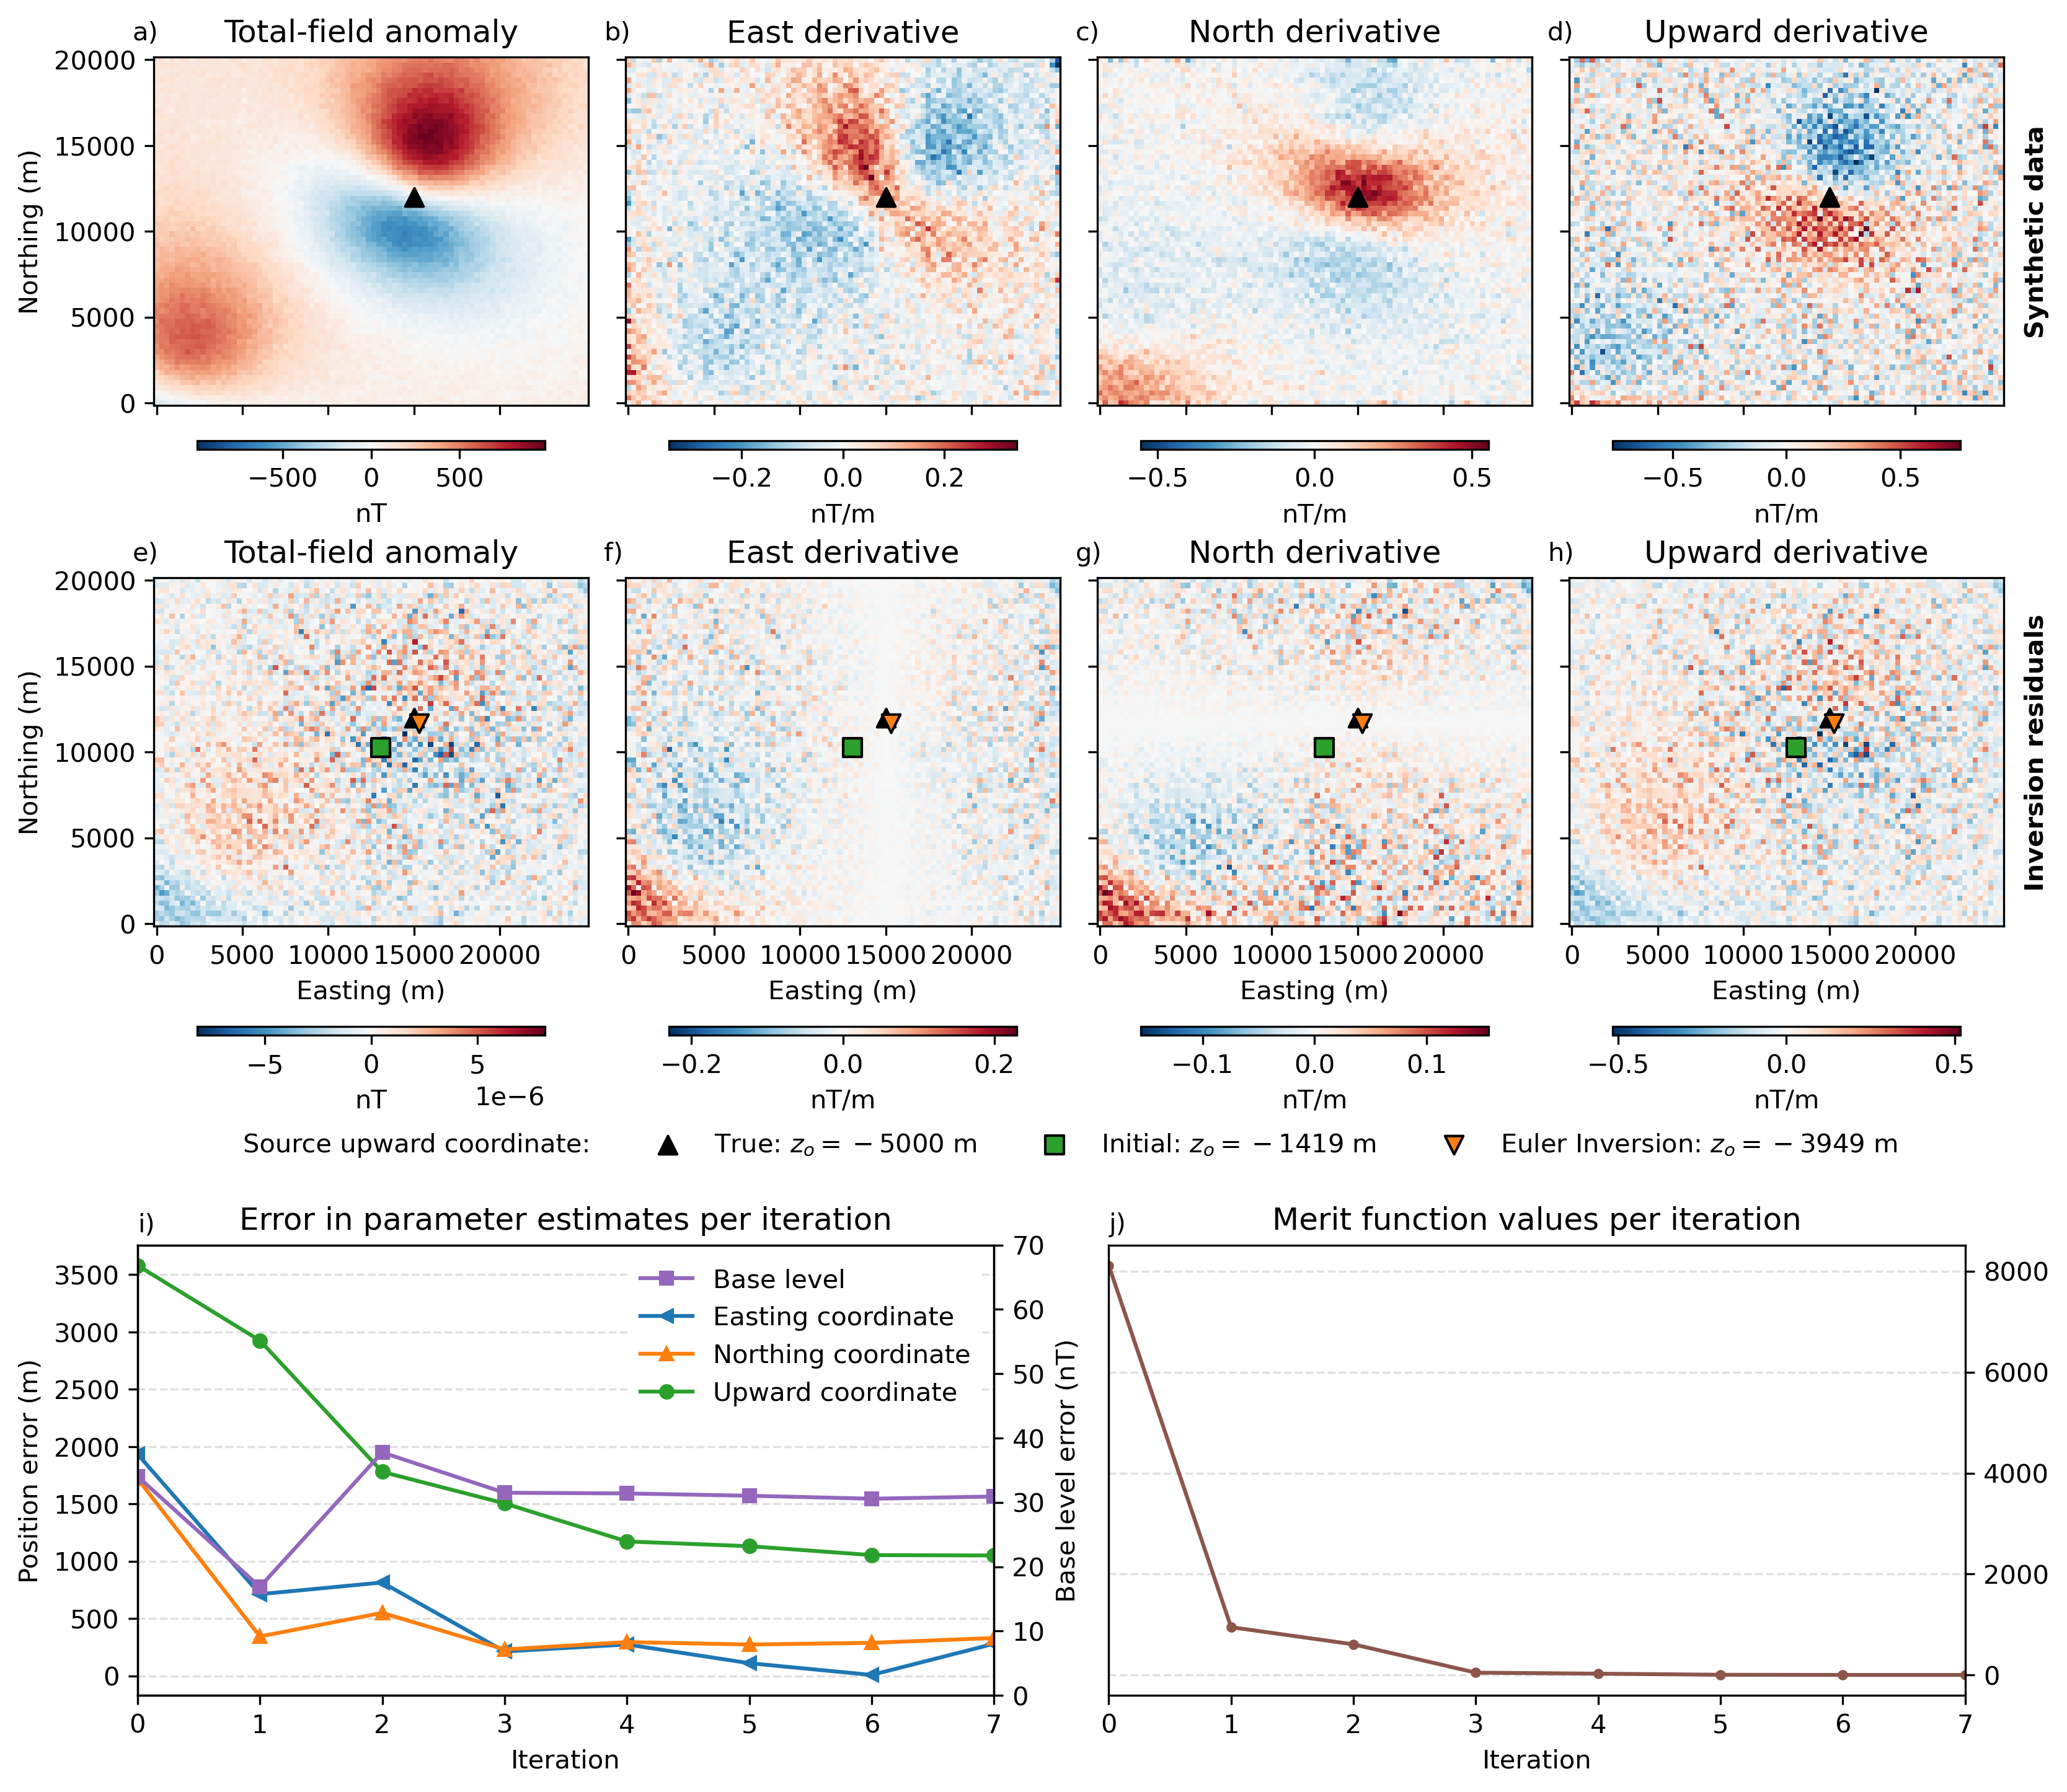
\includegraphics[width=1\linewidth]{figures/synthetic-proof-of-concept.png}
\caption{
  \lipsum[1]
}
\label{fig:proof}
\end{figure}


\subsection{Effect of random noise}

\begin{figure}[tb!]
\centering
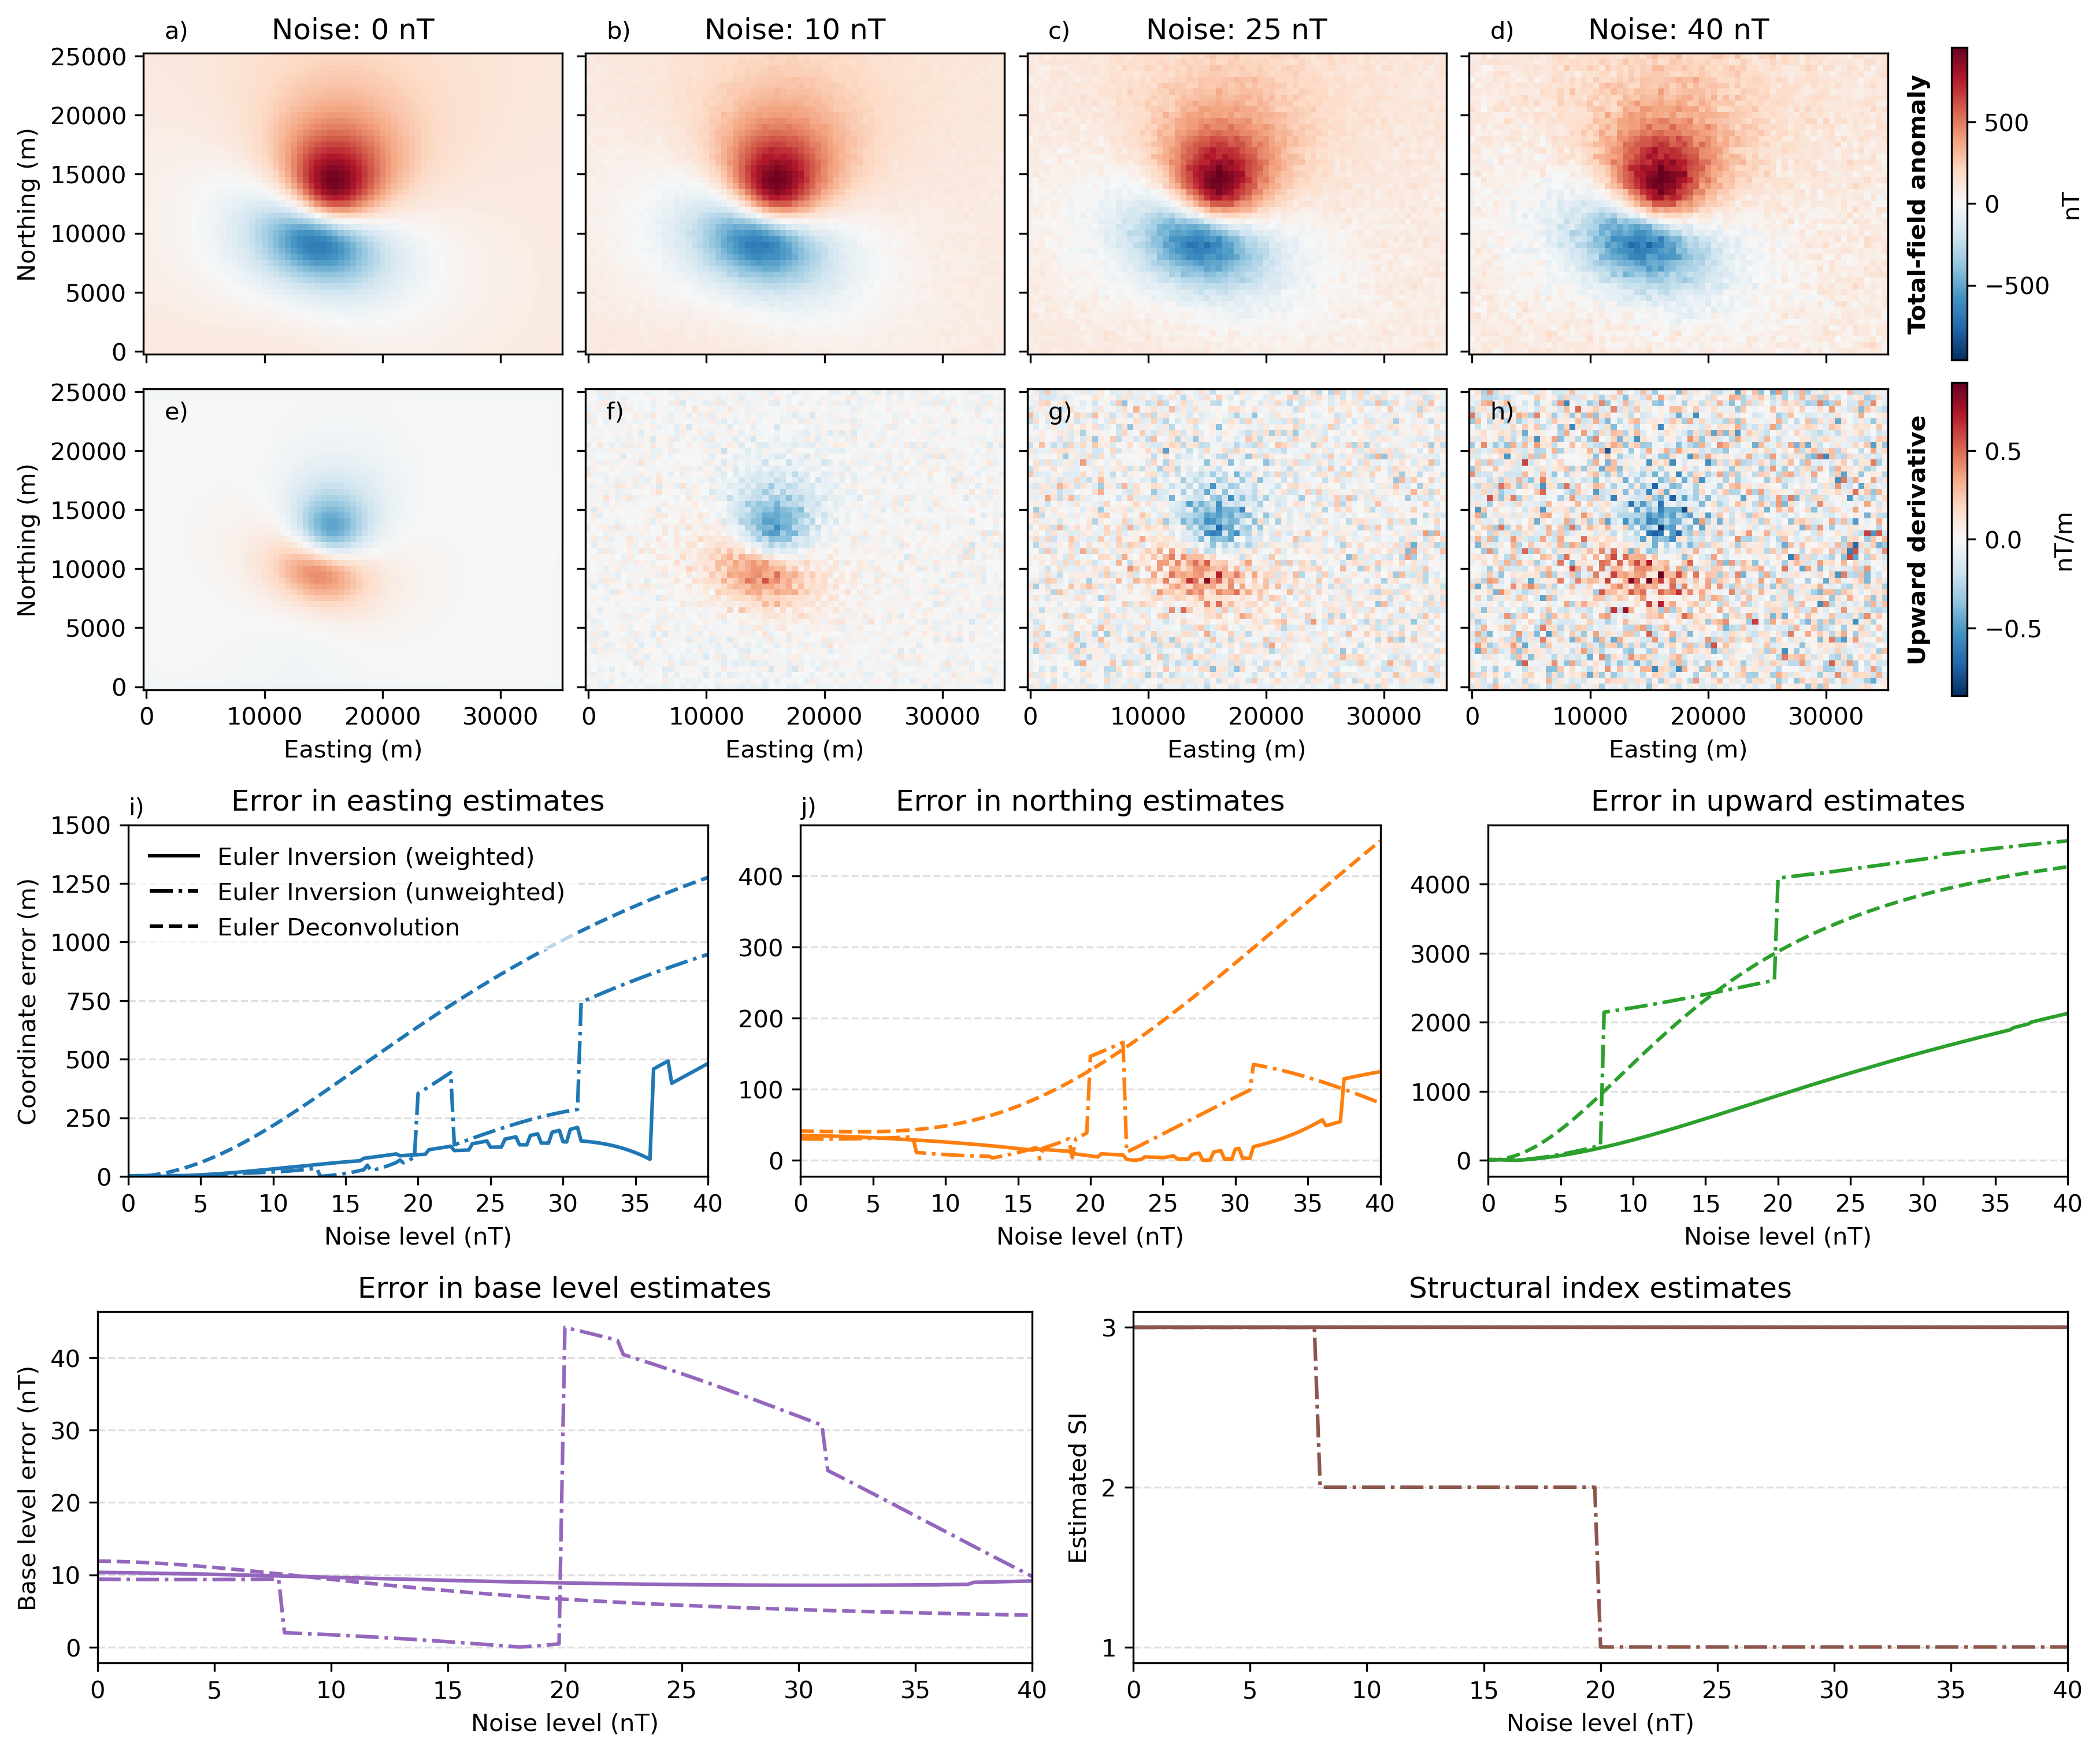
\includegraphics[width=1\linewidth]{figures/synthetic-noise-levels.png}
\caption{
  \lipsum[1]
}
\label{fig:noise}
\end{figure}

\label{sec:si}
\subsection{Effect of SI on multiple sources}

\begin{figure}[tb!]
\centering
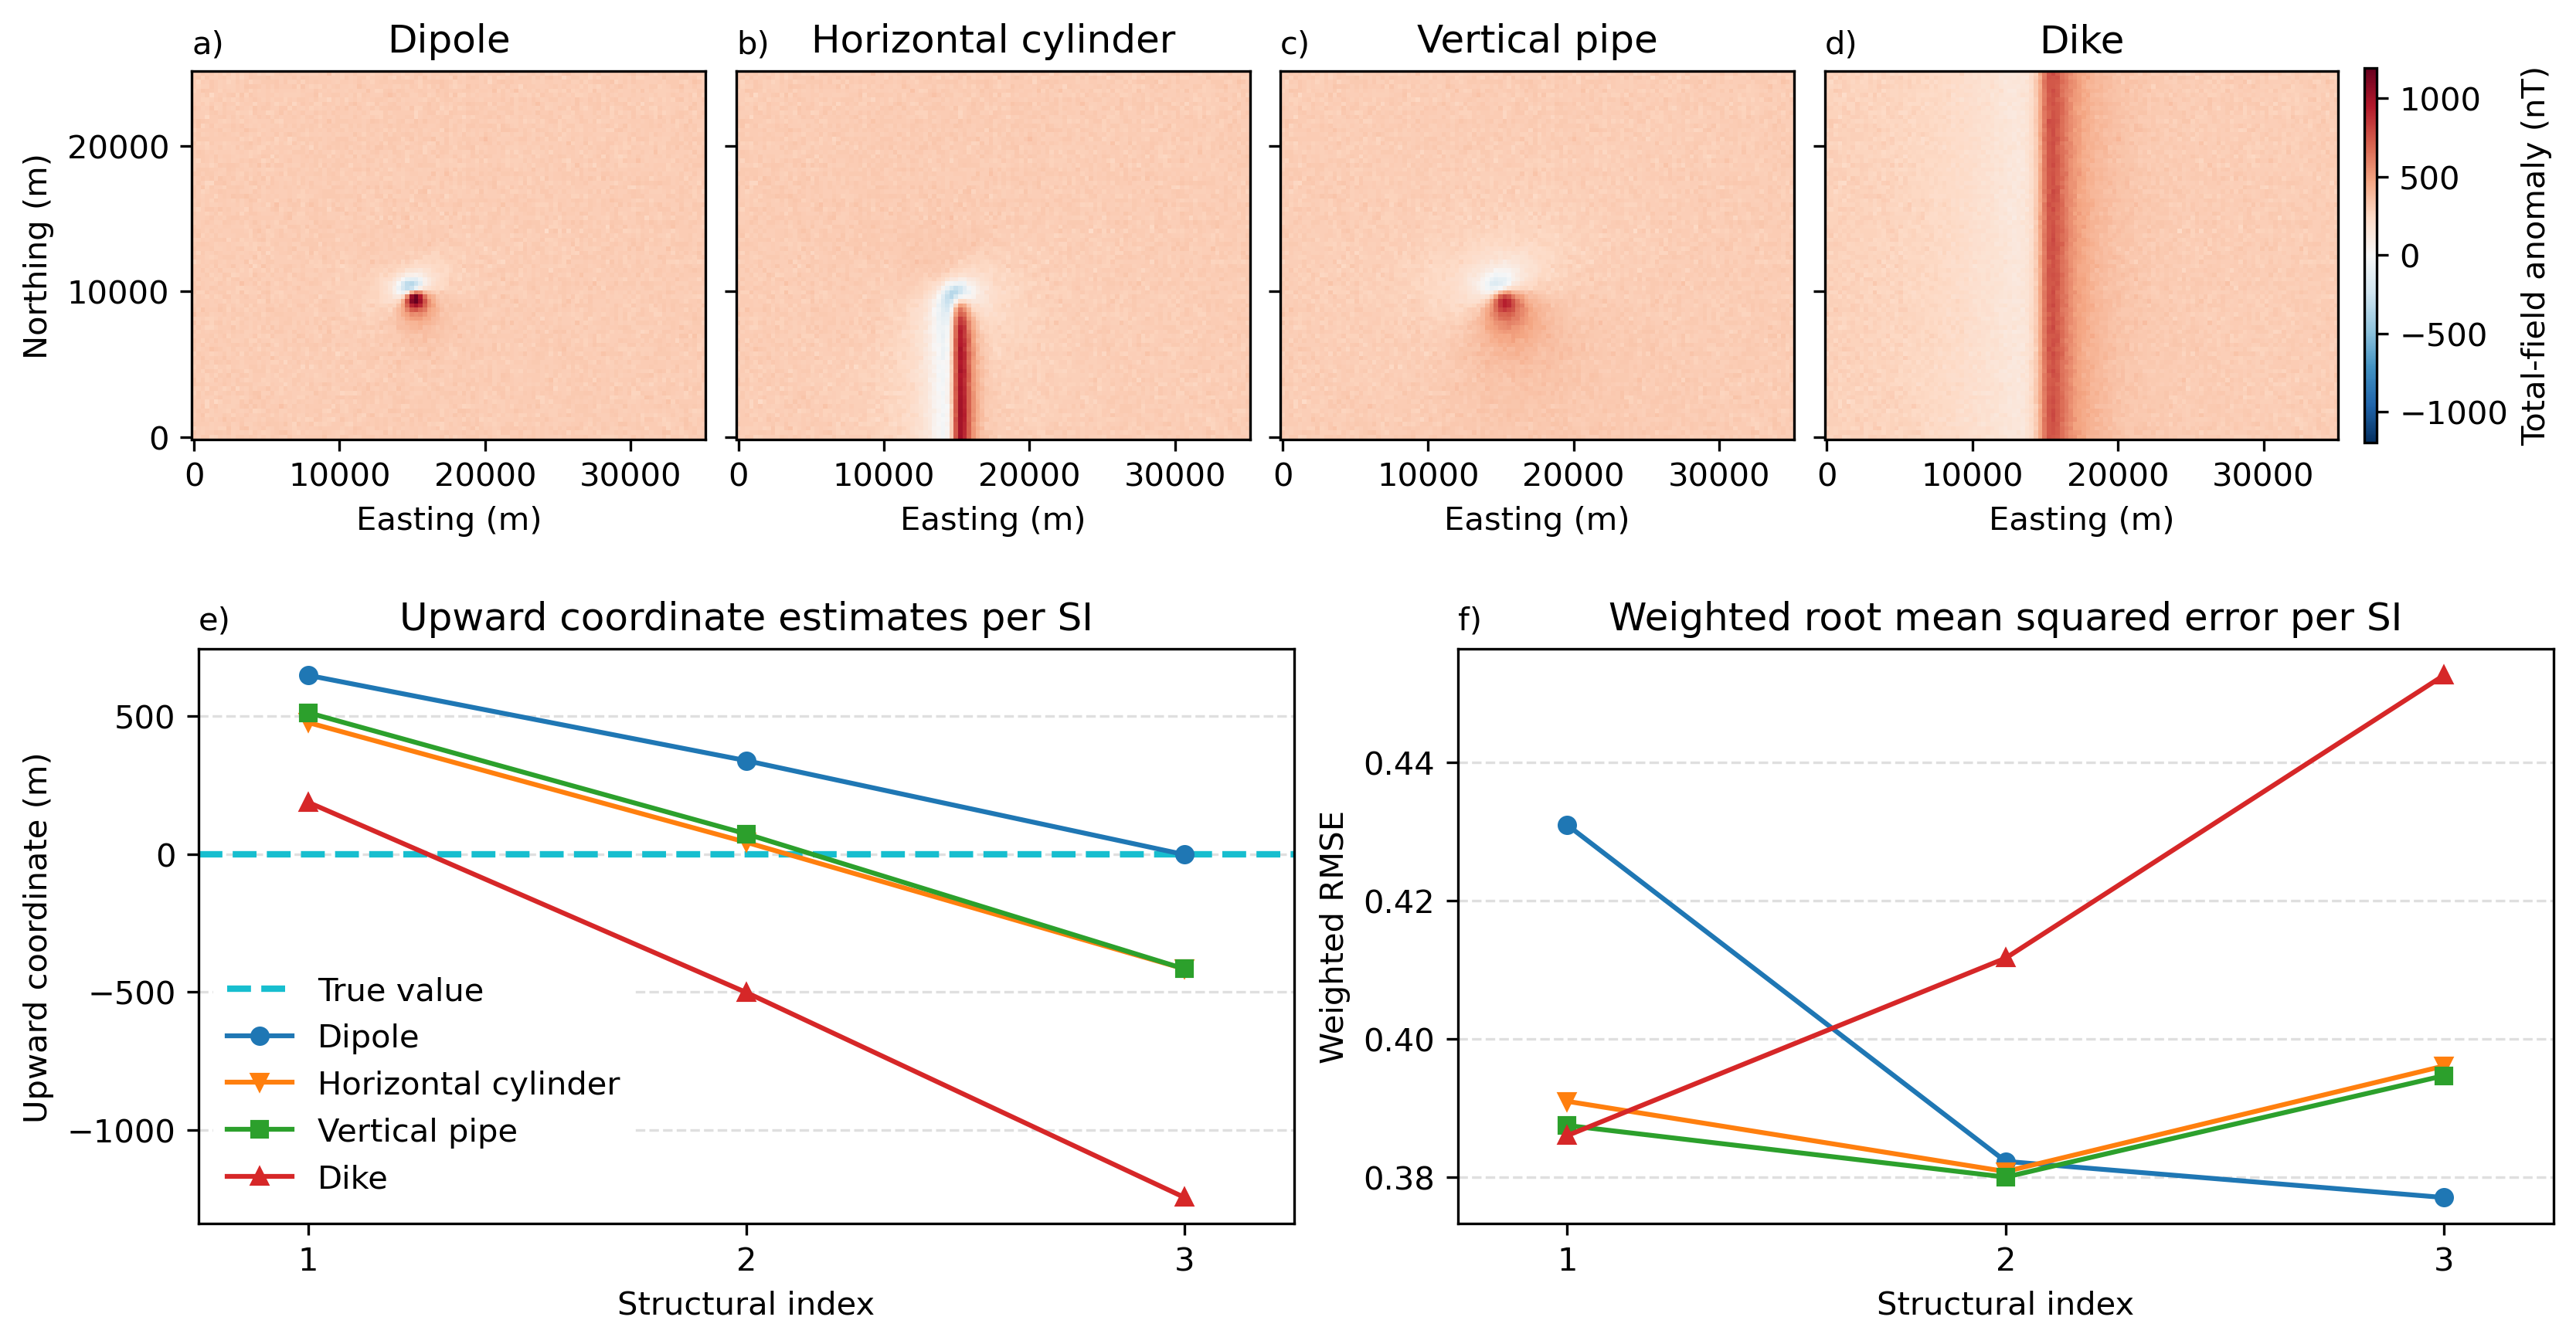
\includegraphics[width=1\linewidth]{figures/synthetic-structural-index.png}
\caption{
  \lipsum[1]
}
\label{fig:si}
\end{figure}

\subsection{Windowing procedure with multiple sources}

\begin{figure}[tb!]
\centering
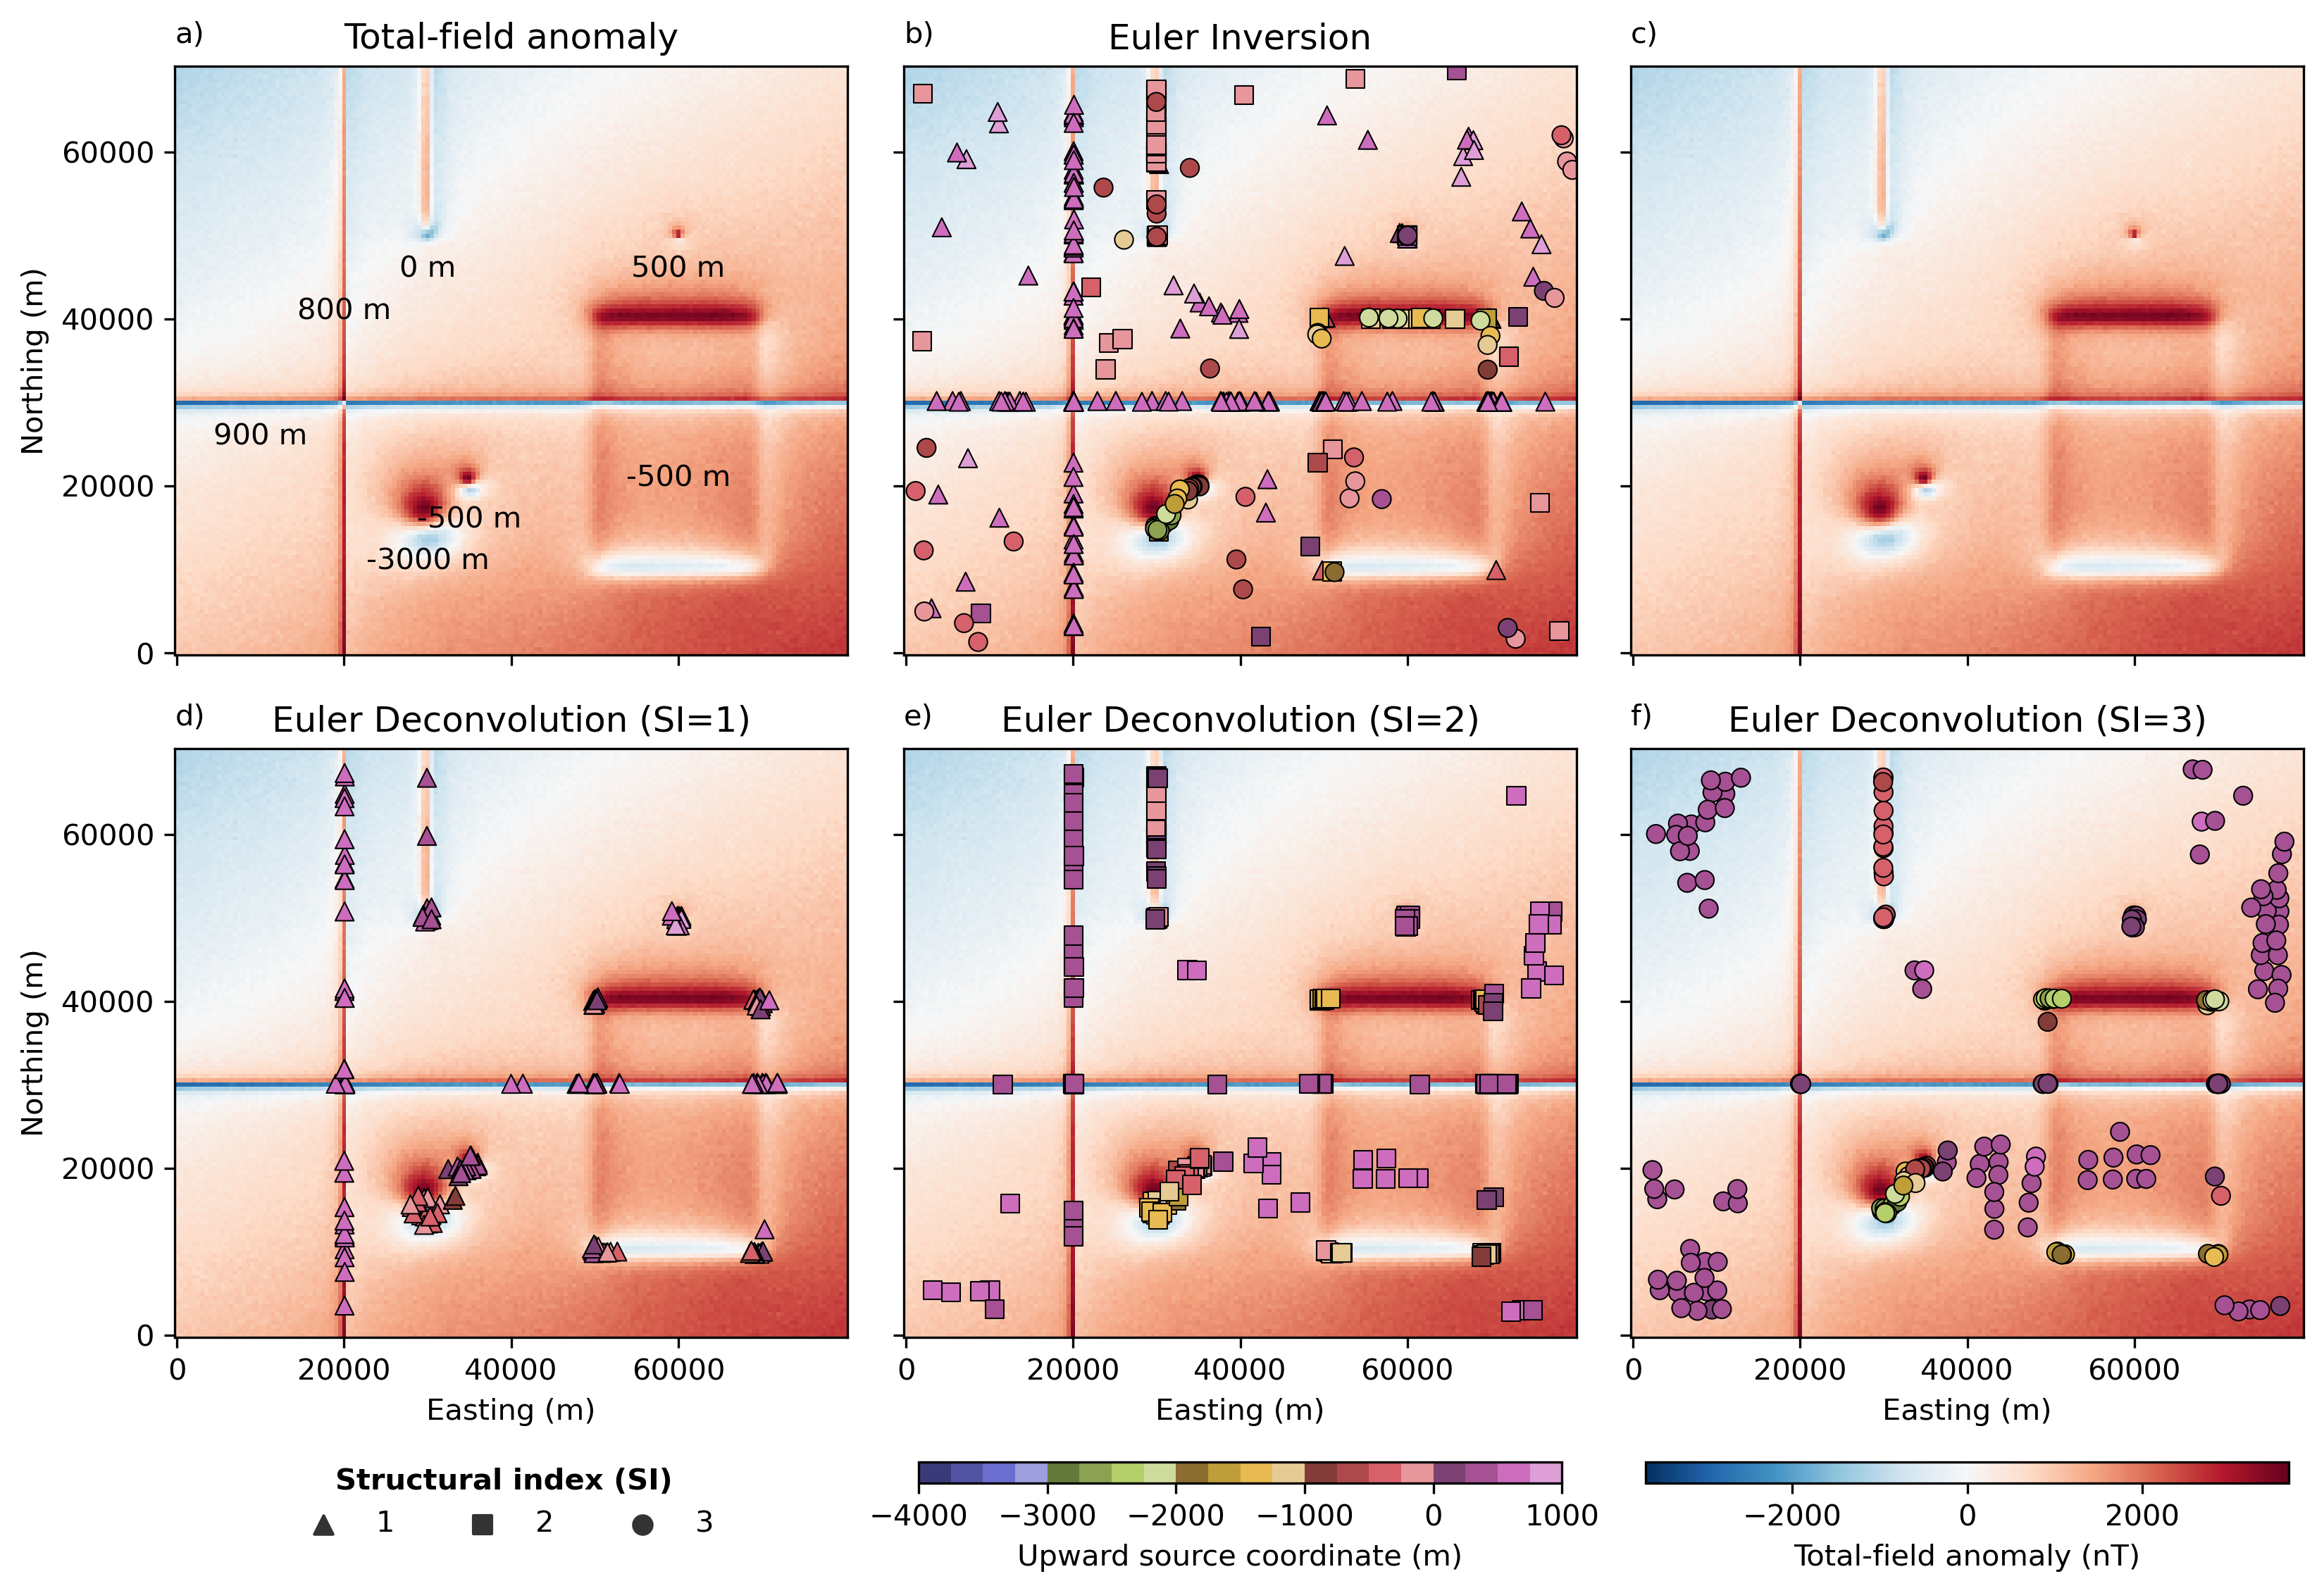
\includegraphics[width=1\linewidth]{figures/synthetic-windows.png}
\caption{
  \lipsum[1]
}
\label{fig:windows}
\end{figure}

\subsection{Aeromagnetic data from Rio de Janeiro}

Gelson and India


%%%%%%%%%%%%%%%%%%%%%%%%%%%%%%%%%%%%%%%%%%%%%%%%%%%%%%%%%%%%%%%%%%%%%%%%%%%%%%%
\section{Conclusion}



%%%%%%%%%%%%%%%%%%%%%%%%%%%%%%%%%%%%%%%%%%%%%%%%%%%%%%%%%%%%%%%%%%%%%%%%%%%%%%%
\section{Open research}

The Python source code and data used to produce all results and figures
presented here are available at \url{https://github.com/\GitHubRepository} and
\url{https://doi.org/\ArchiveDOI} [CITE SOURCE ARCHIVE] under the CC-BY license
and the MIT open-source license.

Here we should cite all of the main software used, like Jupyter, numpy, scipy,
matplotlib, Fatiando, etc.

Cite any data sources as well.



%%%%%%%%%%%%%%%%%%%%%%%%%%%%%%%%%%%%%%%%%%%%%%%%%%%%%%%%%%%%%%%%%%%%%%%%%%%%%%%
\section{Acknowledgements}

We are indebted to the developers and maintainers of the open-source software
without which this work would not have been possible.
Acknowledge any non-author contributors to this study.
Statement about funding.

% Thank the editors and reviewers after review.
